\documentclass[
		pdftex,
		a4paper,	% page format A4
		12pt,		% font size 12pt 
		DIV=calc,
		oneside,	% enable one side
		BCOR5mm,	% add additional padding
		english,	% set language to english
		toc=bibliography,	% include bibliography in TOC
		halfparskip,
		chapterprefix,
		numbers=noenddot,
		titlepage
	]
	{scrbook}   
% ----- weitere Optionen 
%draft,			% Entwurfsmodus zum Anzeigen zu leerer/voller Boxen 
%DIV=calc
%DIV12,			% Seitengröße (siehe Koma Skript Dokumentation !) 
%BCOR5mm,		% Zusätzlicher Rand auf der Innenseite 
%twoside,		% Seitenränder werden an doppelseitig angepasst 
%fleqn,			% Formeln werden linksbündig (und nicht zentriert) angezeigt 
%titlepage,		% Titel wird in einer 'titlepage' Umgebung gesetzt 
%bigheadings,	% Große Überschriften (normal, small-headings) 
%halfparskip-	% Absatz wird nicht eingerückt, dafür aber um eine halbe Zeile nach unten gerückt
%
%---------------------------------------------------
%----- Packages
%---------------------------------------------------
%
\usepackage[
		style=numeric,
		citestyle=numeric,
		maxalphanames=1,
		maxcitenames=2,
		backend=bibtex,
		doi=false,
		isbn=false,
		url=false
	]
	{biblatex}
\usepackage[
		font=small,
		format=plain,
		labelfont=bf,
		up,
		textfont=normal,
		justification=justified,
		singlelinecheck=false
	]
	{caption}
\usepackage{subcaption}
\usepackage{standalone}
\usepackage{lscape}
\usepackage[T1]{fontenc} 
\usepackage[utf8]{inputenc}
\usepackage[english]{babel} 
\usepackage{ae} 
\usepackage{epigraph}
\usepackage{acronym}
\usepackage[toc,page]{appendix}
\usepackage{fancyhdr} % Define simple headings 
\usepackage{xcolor}
\usepackage{url}
\usepackage{listings}
\usepackage{vmargin} % Adjust margins in a simple way
\usepackage{color}
\usepackage{colortbl}
\usepackage{amsmath}
\usepackage{amssymb}
\usepackage{csquotes}
\usepackage{wrapfig} % Paket zur Positionierung einbinden
\usepackage[pdftex]{graphicx}
\usepackage{pgfplots}  
\usepackage{smartdiagram}
\usepackage{metalogo}
\usetikzlibrary{mindmap,trees}
%\usepackage{dtklogos}
\usepackage{hyperref} % turn all your internal references into hyperlinks
%\usepackage[pdfstartview=FitH,pdftitle={<<Titel der Arbeit>>}, pdfauthor={<<Autor>>}, pdfkeywords={<<Schlüsselwörter>>}, pdfsubject={<<Titel der Arbeit>>}, colorlinks=true, linkcolor=black, citecolor=black, urlcolor=black, hypertexnames=false, bookmarksnumbered=true, bookmarksopen=true, pdfborder = {0 0 0}]{hyperref}
%
% table settings 
\usepackage{booktabs}  
\usepackage{tabularx}
\usepackage{array}   
\usepackage{float}
\usepackage{rotating}
\usepackage{longtable}
\usepackage{pdflscape}
\usepackage{multirow} %multi row
\usepackage{rotating} %for rotating table
\usepackage{color}
\usepackage{adjustbox}

%---------------------------------------------------
%----- Bibliography setup
%---------------------------------------------------
%
%\bibliographystyle{alpha}  % citation style
\bibliography{references} % bib file

% the following is needed for syntax highlighting
  
\definecolor{dkgreen}{rgb}{0,0.6,0}
\definecolor{gray}{rgb}{0.5,0.5,0.5}
\definecolor{mauve}{rgb}{0.58,0,0.82}

\definecolor{git_keyword}{HTML}{000000} 
\definecolor{git_key}{HTML}{108888}
\definecolor{git_string}{HTML}{DD1144}
\definecolor{git_tag}{HTML}{121289}
\definecolor{git_attribute}{HTML}{0A8585}
 
\lstdefinelanguage{JSON}{
	keywords={false,true},
	alsoletter=0123456789.,
  	sensitive=false,
  	morecomment=[l]{//},
  	morecomment=[s]{/*}{*/},
  	morestring=[b]',
  	morestring=[b]",
  	keywordstyle=\color{git_key}\bfseries,
    commentstyle=\color{git_string},
	stringstyle=\color{git_string},
}

\lstdefinelanguage{HTML}{
    sensitive=true,
    keywords=[1]{svg, g, path, image},
    otherkeywords={<, \/>, >},   
    keywords=[2]{class, xmlns, xmlns:xlink, xlink:href, width, height, d, x, y},   
    morecomment=[l]{//},
    morecomment=[s]{/*}{*/},
    morecomment=[s]{<!}{>},
    morestring=[b]',
    morestring=[b]",    
    alsoletter={-},
    alsodigit={:},
    keywordstyle=[1]\color{git_tag}\bfseries,
   	keywordstyle=[2]\color{git_attribute},
    commentstyle=\color{git_string},
	stringstyle=\color{git_string},
}

\lstset{
   	backgroundcolor=\color{white},
   	frame=tb,
   	rulecolor=\color{darkgray},    
   	basicstyle=\footnotesize,
   	extendedchars=true,
   	showstringspaces=false,
   	showspaces=false,
   	showtabs=false,
   	numbers=none,
   	tabsize=2,
   	breaklines=true,
   	captionpos=b
}

%
%---------------------------------------------------
%----- PDF and document setup
%---------------------------------------------------
%
\setlength{\parskip}{6pt}
\hypersetup{
	pdftitle={Link the World},  % please, add the title of your thesis
    pdfauthor={Andre Breitenfeld},   % please, add your name
    pdfsubject={Master thesis, Institute of Computer Science, Freie Universität Berlin}, % please, select the type of this document
    pdfstartview={FitH},    % fits the width of the page to the window
    pdfnewwindow=true, 		% links in new window
    colorlinks=false,  		% false: boxed links; true: colored links
    linkcolor=red,          % color of internal links
    citecolor=green,        % color of links to bibliography
    filecolor=magenta,      % color of file links
    urlcolor=cyan           % color of external links
}
%
%---------------------------------------------------
%----- Customize header and footer\pagestyle{fancy} 
%---------------------------------------------------

\fancypagestyle{plain}{ % 'plain' page style (used for first page of chapter)
  \fancyhf{} % clear all header and footer fields
  \fancyfoot[R]{\thepage}
}

\pagestyle{fancy}

\fancyhf{}  % delete all existing header formating
\fancyhead[R]{\leftmark}  % represent the current chapter heading in uppercase
\renewcommand{\chaptermark}[1]{ % adapt the shown chapter name: show it in lower case and with chapter number 
\markboth{\thechapter.\ #1}{}}   

%\fancyhead[RO]{\rightmark}   % % represent the current section heading in uppercase 
\renewcommand{\sectionmark}[1]{% adapt the shown section name: show it in lower case and with section number 
\markboth{\thesection.\ #1}{}}

\renewcommand{\headrulewidth}{0pt} % remove lines from header
\renewcommand{\footrulewidth}{0pt} % remove lines from header

\newcommand{\tab}{\hspace*{2em}}

% Source http://tex.stackexchange.com/a/32690
\newcolumntype{R}[2]{%
    >{\adjustbox{angle=#1,lap=\width-(#2)}\bgroup}%
    l%
    <{\egroup}%
}
\newcommand*\rot{\multicolumn{1}{R{45}{1em}}}% no optional argument here, please!

\fancyfoot{} % delete all existing footer formating
\fancyfoot[R]{\thepage} 

%%%%%%%%%%%%%%%%%%%%%%%%%%%%%%%%%%%%%%%%%%%%%%%%%%%%%%%%%%%%%%%%%%%%%%%%%%%%%%
% ---- Namen der Links im Dokument
%\addto\captionsngerman{\renewcommand{\figurename}{\small{\textbf{Abb.}}}}
%\addto\captionsngerman{\renewcommand{\tablename}{Tab.}}
%\addto\captionsngerman{\captionsetup{figurewithin = section}}
%\addto\captionsngerman{\captionsetup{font=small, labelfont=bf}}

%
%---------------------------------------------------      
%----- Settings for word separation  
%---------------------------------------------------      
% Help for separation (from package babel, section 22)):
% In german package the following hints are additionally available:
% "- = an explicit hyphen sign, allowing hyphenation in the rest of the word
% "| = disable ligature at this position. (e.g., Schaf"|fell)
% "~ = for a compound word mark without a breakpoint (e.g., bergauf und "~ab)
% "= = for a compound word mark with a breakpoint, allowing hyphenation in the composing words
% "" = like "-, but producing no hyphen sign (e.g., und/""oder)
%
% Describe separation hints here:
\hyphenation{
% Pro-to-koll-in-stan-zen
% Ma-na-ge-ment  Netz-werk-ele-men-ten
% Netz-werk Netz-werk-re-ser-vie-rung
% Netz-werk-adap-ter Fein-ju-stier-ung
% Da-ten-strom-spe-zi-fi-ka-tion Pa-ket-rumpf
% Kon-troll-in-stanz
}

%%%%%%%%%%%%%%%%%%%%%%%%%%%%%%%%%%%%%%%%%%%%%%%%%%%%%%
% The content part of the document starts here! %%
%%%%%%%%%%%%%%%%%%%%%%%%%%%%%%%%%%%%%%%%%%%%%%%%%%%%%%

\begin{document}
\frontmatter 

%\pagenumbering{alph} % even though, these page numbers are not visible there are necessary to have unique page numbers 
% ---------------------------------------------------
% ----- Title page of the template
% ----- for Bachelor-, Master thesis and class papers
% ---------------------------------------------------
%  Created by C. Müller-Birn on 2012-08-17, CC-BY-SA 3.0.
%  Freie Universität Berlin, Institute of Computer Science, Human Centered Computing. 
%
\begin{titlepage}

\title{
{\small Master Thesis, Institute of Computer Science, Freie Universität Berlin}\\
{\small Biorobotics Lab, Intelligent Systems and Robotics}\\
[6ex]
{\LARGE Temporal Analysis of\\ Honey Bee Interaction Networks\\Based on Spatial Proximity\\}
\vspace{2ex}
\begin{tikzpicture}[node distance=1cm]
  \node[regular polygon, regular polygon sides=6, shape aspect=0.5, minimum width=1.5cm, minimum height=1cm, draw] (reg) {};
\end{tikzpicture}\\
}

\author{
{\emph{\normalsize Alexa Schlegel}}\\
{\normalsize Matriculation number: 4292909}\\
{\normalsize alexa.schlegel@fu-berlin.de}\\ 
[15ex]   
{\normalsize Supervisor: Prof. Dr. Tim Landgraf, Freie Universität Berlin}\\
{\normalsize Second Supervisor: Dr. Philipp Hövel, Technische Universität Berlin}\\
}
\vspace{6ex}
\date{\normalsize Berlin, \today}
 
\maketitle  


\end{titlepage}
% ---------------------------------------------------
% ----- Declaration of the template
% ----- for Bachelor-, Master thesis and class papers
% ---------------------------------------------------
%  Created by C. Müller-Birn on 2012-08-17, CC-BY-SA 3.0.
%  Freie Universität Berlin, Institute of Computer Science, Human Centered Computing. 
%
\pagestyle{empty}

\subsection*{Eidesstattliche Erklärung}

Ich versichere hiermit an Eides Statt, dass diese Arbeit von niemand anderem als meiner Person verfasst worden ist. Alle verwendeten Hilfsmittel wie Berichte, Bücher, Internetseiten oder ähnliches sind im Literaturverzeichnis angegeben, Zitate aus fremden Arbeiten sind als solche kenntlich gemacht. Die Arbeit wurde bisher in gleicher oder ähnlicher Form keiner anderen Prüfungskommission vorgelegt und auch nicht veröffentlicht.
\par\bigskip  
\noindent Berlin, den \today

\vspace{1.2cm}

\noindent Alexa Schlegel

\cleardoublepage
%*******************************************************
% Dedication
%*******************************************************
\thispagestyle{empty}
%\phantomsection 

\pdfbookmark[1]{Dedication}{Dedication}

\vspace*{3cm}

\begin{center}
    Everything we hear is an opinion, not a fact. \\ Everything we see is a perspective, not the truth.  \\ \medskip
    --- Marcus Aurelius 
\end{center}

\medskip

\begin{center}
    Dedicated to my parents and my brother.
\end{center}

%---------------------------------------------------
%----- Abstracts in English and German   
%---------------------------------------------------

% ---------------------------------------------------
% ----- Abstract (English)
% ---------------------------------------------------
%  Freie Universität Berlin, Institute of Computer Science, Human Centered Computing. 
%
\pagestyle{empty}
\providecommand{\keywords}[1]{\textbf{\textit{Keywords---}} #1}

\subsection*{Abstract}
The BeesBook system automatically tracks individual honey bees inside a hive over their entire life and provides a high-resolution dataset of bee movements of a single colony.
This thesis focuses on the inference of interaction networks, by implementing a network pipeline.
Spatial proximity is using as an indicator for interactions between bees.
Social network analysis methods were applied to investigate the static and dynamic properties of the resulting social networks of honey bees on a global, intermediate and local level.
The resulting networks were characterized by a low hierarchical structure and a high density.
The global structure of the colony seems to be stable over time.
The local structure is highly dynamic, as bees change communities as they age.
Communities in the honey bee network represent age groups with a high spatial fidelity.
The findings are in line with established state of research that a colonies organization is shaped by the age-based task division of individuals.
The results of the analysis validate the implemented pipeline and inferred networks and consequently provide an excellent foundation for future work focusing more on temporal network analysis aspects.

\keywords{social insects, spatial proximity network, social network, interaction network, honey bee, behavioural tracking, Apis mellifera, community detection, social network analysis}

\cleardoublepage

% ---------------------------------------------------
% ----- Abstract (German) of the template
% ----- for Bachelor-, Master thesis and class papers
% ---------------------------------------------------
%  Created by C. Müller-Birn on 2012-08-17, CC-BY-SA 3.0.
%  Freie Universität Berlin, Institute of Computer Science, Human Centered Computing. 
%
\pagestyle{empty}

\subsection*{Zusammenfassung}
ein abstract auf deutsch

\cleardoublepage  
                                          
%---------------------------------------------------
%----- Table of content   
%---------------------------------------------------
\tableofcontents
%\setcounter{tocdepth}{3}   % reduce the included sections in the table of content

%---------------------------------------------------
%----- Main part
%---------------------------------------------------
\mainmatter

\pagestyle{fancy} 

%%%%%%%%%%%%%%%%%%%%%%%%%%%%%%%%%%%%%%%%%%%%%%%%%%%%%%%%%%%%%%%%%%%%%%%%%%%%%%%
%%%%%%%%%%%%%%%%%%%%%%%%%%%%%%%%%%%%%%%%%%%%%%%%%%%%%%%%%%%%%%%%%%%%%%%%%%%%%%%
%%%%%%%%%%%%%%%%%%%%%%%%%%%%%%%%%%%%%%%%%%%%%%%%%%%%%%%%%%%%%%%%%%%%%%%%%%%%%%%
%%%%%%%%%%%%%%%%%%%%%%%%%%%%%%%%%%%%%%%%%%%%%%%%%%%%%%%%%%%%%%%%%%%%%%%%%%%%%%%
\chapter{Introduction}
\label{ch:intro}
%%%%%%%%%%%%%%%%%%%%%%%%%%%%%%%%%%%%%%%%%%%%%%%%%%%%%%%%%%%%%%%%%%%%%%%%%%%%%%%
%%%%%%%%%%%%%%%%%%%%%%%%%%%%%%%%%%%%%%%%%%%%%%%%%%%%%%%%%%%%%%%%%%%%%%%%%%%%%%%
%%%%%%%%%%%%%%%%%%%%%%%%%%%%%%%%%%%%%%%%%%%%%%%%%%%%%%%%%%%%%%%%%%%%%%%%%%%%%%%
%%%%%%%%%%%%%%%%%%%%%%%%%%%%%%%%%%%%%%%%%%%%%%%%%%%%%%%%%%%%%%%%%%%%%%%%%%%%%%%

A social insect society is formed by thousands of individuals, which continuously move and interact with each other inside a dark nest. 
Honey bees are organized in colonies, which form a complex and dynamical system.
Observing individual honey bees and their interactions with each other is, therefore, vital for understanding collective behavior and the organization of tasks within the colony.

Within the BeesBook project of the Biorobotics Lab of Freie Universität Berlin~\textcite{wario2015automatic} developed technologies to automatically track all individuals of a honey bee (Apis mellifera) colony, that are inside the honeycomb.

Shortly after hatching, each bee is marked on their thorax by using circular 12-bit tags (figure~\ref{fig:markers}) and then added to the observation colony. Four cameras observe the comb over a period of nine weeks, by capturing approximately three frames per second. An image analysis pipeline evaluates each frame automatically. The resulting data set contains, for each frame, the exact position of each detected bee on the honeycomb, and its age.

In this thesis, worker-worker interaction networks, based on spatial proximity, are derived from the described data set. Each node in the network is a bee, and a link between two nodes results if two bees are located close to each other over a specified period.
The networks are time-aggregated, which means one network represents the data of multiple frames.

After extracting the temporal networks, social network analysis methods are applied to determine the characteristics of the resulting networks and its communities.

\begin{figure}[htb]
	\centering
	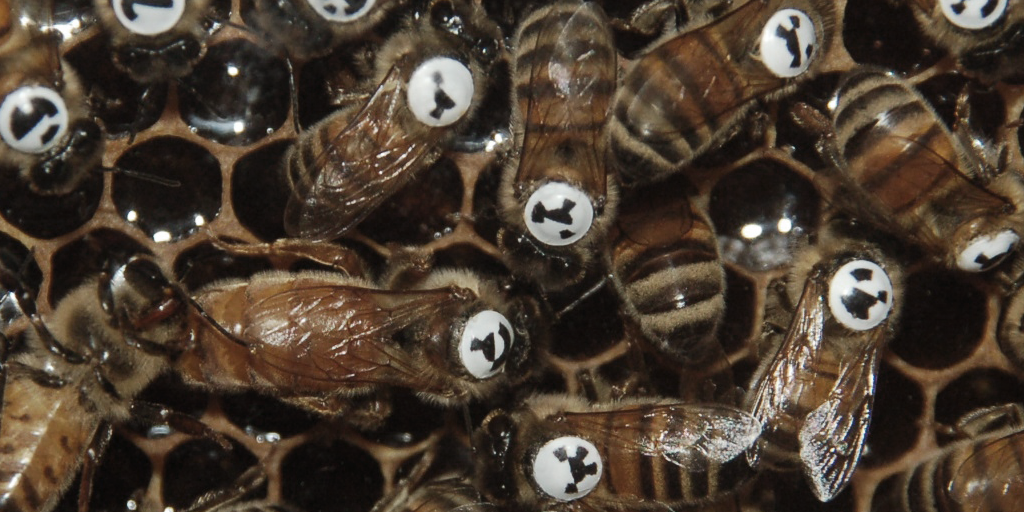
\includegraphics[width=1.0\textwidth]{Figures/markers}
	\caption{Tagged bees inside the observation hive.}
	\label{fig:markers}
\end{figure}

%%%%%%%%%%%%%%%%%%%%%%%%%%%%%%%%%%%%%%%%%%%%%%%%%%%%%%%%%%%%%%%%%%%%%%%%%%%%%%%
%%%%%%%%%%%%%%%%%%%%%%%%%%%%%%%%%%%%%%%%%%%%%%%%%%%%%%%%%%%%%%%%%%%%%%%%%%%%%%%
\section{Motivation}
%%%%%%%%%%%%%%%%%%%%%%%%%%%%%%%%%%%%%%%%%%%%%%%%%%%%%%%%%%%%%%%%%%%%%%%%%%%%%%%
%%%%%%%%%%%%%%%%%%%%%%%%%%%%%%%%%%%%%%%%%%%%%%%%%%%%%%%%%%%%%%%%%%%%%%%%%%%%%%%

Colonies of social insects consist of a vast number of individuals. Due to technical and observational limitations, most studies in the field of animal social network analysis, related to insects, analyze only a small subset of a colonies' life.
Usually, the reduction is carried out on three levels (1) time and resolution, (2) space, and (3) number of individuals.


[TODO: umarbeiten!!!, einzelne Studien müssen in related work, (A) method/approach: network analysis, network properties and communities; (B) animals: focus bees, but also considering social insects studies; (C) tracking methods: manual tracking and automatic tracking; automatic tracking, more inclusive, temporal development, dadurch Mehrwert, d.h. gap of knowledge im Bereich: Social Network Analysis von Honey Bees with automatic tracking and long term development, hm... Studies in den anderen Bereichen (automatic tracking and social insects, manual tracking bees, manual tracking of social insects, with network science approach already exists). Automatic tracking allows shifting more towards the temporal and dynamic investigation.]

Labeling only a subset of the colonies individuals, a short observation period, low res\-olution and manually extracting information from photos or videos is very common in behavioral sciences~\cite{naug2008structure, quevillon2015social}.

\textcite{baracchi2014socio} observed 300 bees out of a colony with 4000 individuals over a period of ten hours. One of the two sides of the hive was observed by taking a photo each minute. Coloured numbered discs were used for individually marking bees. The analysis of a weighted and undirected worker-worker interaction network revealed a highly compartmentalized structure inside the honey bee colony. Depending on the age, bees occupy different areas of the comb and correspond to different tasks. Also, the contact is limited within groups. \textcite{blonder2011time} color painted all individuals of ant colonies (size 6-90 for each colony) and filmed the colonies for 30 minutes. Interactions between individuals were manually extracted by watching the videos. Using time-ordered (dynamic) networks they analyzed the temporal and spatial dynamics of information flow.

Recently, automated tracking of insects has become technically feasible~\cite{wario2015automatic, crall2015beetag, fiala2005comparing}.
Using automated high resolution tracking data, which includes all individuals of the complete comb over a long time period allows for more advanced analysis focusing on temporal dynamics.
\textcite{mersch2013tracking} automatically tracked all individuals of six ant colonies over a period of 41 days. Applying the Infomap community detection algorithm to the physical contact networks for each day, revealed three distinct and robust groups. Each group represents a functional behavioral unit, with individuals changing groups as they age.

The majority of social insect interaction networks studies, due to previously technical limitations, aggregate temporal tracking data into a single static network~\cite[Chapter~15]{krause2014animal}.
Automatic tracking allows shifting more towards the temporal and dynamic investigation.


\section{Research Goal}
The aim of this thesis is to investigate whether the provided data set of tracked honey bees is useful for creating worker-worker interaction networks using spatial proximity as an indicator for interactions between bees. Thus, I need to implement a pipeline to extract networks out of the given data set. Furthermore, I want to find out if the resulting networks are suitable for social network analysis.

I want to achieve my research goals by answering the following questions:

\begin{enumerate}
\item \emph{Is it possible to infer (temporal) networks with the provided honey bee tracking data?}\\
What challenges and limitations does the data set imply?
What pipeline parameters are necessary?
\item \emph{What kind of worker-worker interaction networks emerge and how are they structured?}\\
What is their topology?
What properties are characteristic and how do they differ from randomly generated networks?
\item \emph{Does the network display a meaningful community structure?}\\
How are the identified communities characterized?
Do they reflect already known colony behavior concerning age and spatial distribution?
\item \emph{How do these communities develop over time?}\\
Are they stable regarding their properties?
How do members move between communities?
\end{enumerate}

This work is meant to be the foundation to answer further more specific biological research questions using a network science approach to study and evaluate the complex system of honey bee colonies and their collective behavior.

\section{Methodology}
The methodology of this thesis follows a standard explorative data analysis procedure, mainly to understand the given data set and estimate its quality. The elaborated characteristics of the dataset are then used to define parameters and the procedure of network extraction. This pipeline is developed, tested and then refined in an iterative process. Test results lead to new or changing functional requirements of the pipeline.

The resulting networks are evaluated using the following approaches:

\begin{itemize}
\item Investigation of pipeline parameters' effects,
\item Quality inspection by examining the age of bees,
\item Comparison with a random graph model,
\item Repeatability of known results and facts concerning community structures.
\end{itemize}

\section{Outline}
This thesis is organized as follows. Chapter~\ref{ch:bg} gives a short introduction into social network analysis (SNA) and defines network measures, terms, and algorithms used throughout this work.
In chapter~\ref{ch:relatedwork}, a brief summary of the current state of research concerning social insect networks, temporal networks and community detection in animal social networks is given.
Chapter~\ref{ch:approach} describes my research approach in general and how the pipeline infers networks out of the given dataset, what steps are needed and what parameters it uses.
Also, I explain and justify what decisions I took during the network analyses and community detection process.
Chapter~\ref{ch:results} reports the results of the network analysis and the characteristics of the extracted communities.
Finally, in chapter~\ref{ch:conclusion} I explore the results, discuss limitations and conclude with directions for future work.

%---------------------------------------------------
%----- Bibliography
%---------------------------------------------------
\printbibliography

%---------------------------------------------------
%----- Directories   
%---------------------------------------------------

\addcontentsline{toc}{chapter}{\listfigurename}
\listoffigures
\clearpage %\cleardoublepage %for openright
\addcontentsline{toc}{chapter}{\listtablename}
\listoftables
\clearpage %\cleardoublepage %for openright
%\lstlistoflistings

%---------------------------------------------------
%----- Appendix   
%---------------------------------------------------
\appendix
\chapter{Appendix Stuff}
\label{ch:appendix}

\begin{table}
\centering
\caption[XXX]{\textbf{XXX} \url{https://docs.google.com/spreadsheets/d/1eKuPU-XmqwrHkS_5-TgS8UnO5O-Hwe1kyRIpareywP4/edit?usp=sharing}}
\label{tab:studies}
\vspace*{5mm}
\begin{tabular}{ccc}
	\toprule
	{}  & TODO & TODO \\
	\midrule

	x & x & x\\
	x & x & x\\
	\bottomrule
\end{tabular}
\end{table}

[TODO: Table with studies related to social insects and bees and manual and automatic tracking.]

[TODO: Figure: Maintance and Faliour Days, also maybe timeline for each camera]

[TODO: ]
\backmatter

\end{document}